\section{analysis}
\label{sec:analysis}

\subsection{Property distributions}
Here we will look at the frequency distributions (histograms) comparing the characteristics of CPSBs, RPSBs an their control galaxies.

We compare the distributions of CPSBs with that of the RPSB sample in terms of S\'ersic index, stellar mass, and redshift. These distributions are taken from the data in Tables \ref{tab:my-CPSBs} and \ref{tab:my-RPSBs}. The frequency distribution histograms are plotted in Figures \ref{fig:Sersic-plot}, \ref{fig:stellar-mass-plot} and \ref{fig:redshift-plot} respectively.

\begin{figure}
    \centering
    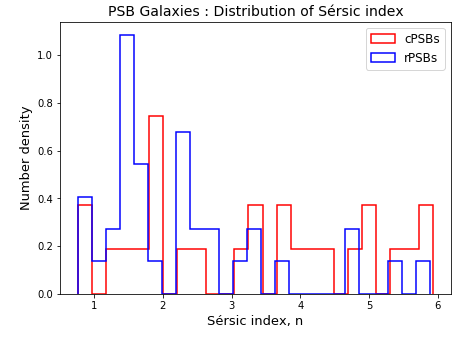
\includegraphics[width=\columnwidth]{images/Seric-index-distribution.png}
    \caption{Distribution of S\'ersic index values.}
    \label{fig:Sersic-plot}
\end{figure}

\begin{figure}
    \centering
    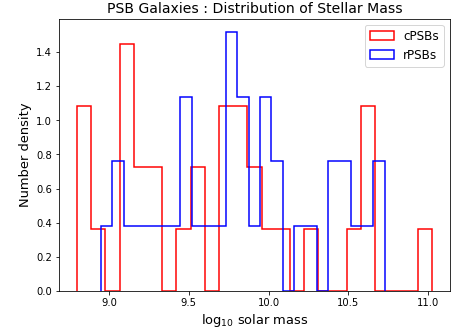
\includegraphics[width=\columnwidth]{images/Stellar-mass-distribution.png}
    \caption{Distribution of Stellar mass.}
    \label{fig:stellar-mass-plot}
\end{figure}

\begin{figure}
    \centering
    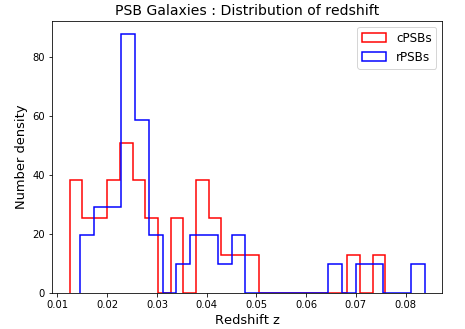
\includegraphics[width=\columnwidth]{images/Redshift-distribution.png}
    \caption{Distribution in redshift.}
    \label{fig:redshift-plot}
\end{figure}

\subsection{The KS-test}
The Kolmogorov-Smirnov test: a statistical test to determine if two samples come from the same underlying distribution. Tests for goodness of fit. Can use \texttt{scipy.stats.kstest}, see for example \url{https://stackoverflow.com/questions/10884668/two-sample-kolmogorov-smirnov-test-in-python-scipy}.

\subsection{The Radon transform}
Describe the principles of the Radon transform, its history and its purpose and relevance to this research. Refer to \cite{2018MNRAS.480.2217S}.

\begin{equation}
    \label{eqn:radon}
    R(\rho,\theta)=\int_{L}{v(x,y) dL} 
\end{equation}

An example of the graphical output of the Radon transform as applied to a synthetic velocity field is shown in Fig. \ref{fig:Radon}.

\begin{figure}
    \centering
   	\includegraphics[width=\columnwidth]{images/RadonPlots/example (4).jpg}
    \caption{Model Radon transform plots from \citet{2018MNRAS.480.2217S}.}
    \label{fig:Radon}
\end{figure}




\begin{figure}
    \centering
   	\includegraphics[width=\columnwidth]{images/RadonPlots/RT-8313-6101-SV+GV-A10.jpeg}
    \caption{Radon transform plots of the stellar velocity (left panel) and gas velocity (right) fields of CPSB of MaNGA PLATEIFU 8131-6101}
    \label{fig:RT_8131-6101}
\end{figure}

\subsection{Smoothed velocity fields}
[This method has already been trialled. Considered as 1st year PhD level. Need to get some references XXX.]